% big ball with 4 small balls (cardinal), gray overlap lenses, black diagonal gaps
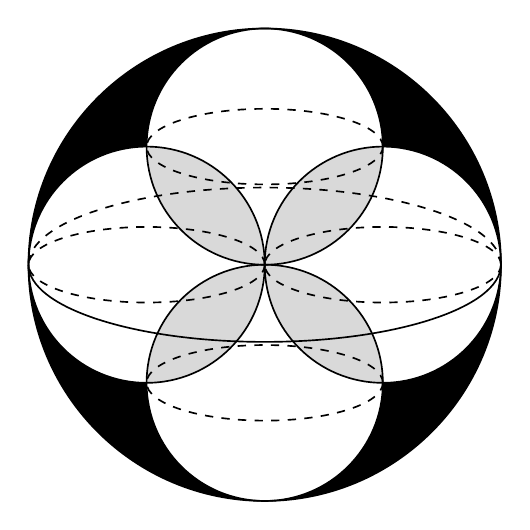
\begin{tikzpicture}[x=1cm,y=1cm,line width=.6pt,font=\normalsize]
\coordinate (O) at (0,0);
\def\R{3}\def\r{1.5}
% black base disc
\fill[black] (O) circle (\R);
% four white small discs (cardinal, radius R/2, centers at distance R/2)
\fill[white] (0,1.5) circle (\r);
\fill[white] (0,-1.5) circle (\r);
\fill[white] (-1.5,0) circle (\r);
\fill[white] (1.5,0) circle (\r);
% gray pairwise overlap lenses around center (clip pairs)
\begin{scope}\clip (0,1.5) circle (\r);\fill[gray!30] (1.5,0) circle (\r);\end{scope}
\begin{scope}\clip (0,1.5) circle (\r);\fill[gray!30] (-1.5,0) circle (\r);\end{scope}
\begin{scope}\clip (0,-1.5) circle (\r);\fill[gray!30] (1.5,0) circle (\r);\end{scope}
\begin{scope}\clip (0,-1.5) circle (\r);\fill[gray!30] (-1.5,0) circle (\r);\end{scope}
% outlines
\draw (O) circle (\R);
\draw (0,1.5) circle (\r);
\draw (0,-1.5) circle (\r);
\draw (-1.5,0) circle (\r);
\draw (1.5,0) circle (\r);
% big equator: solid front, dashed back
\draw (-3,0) arc (180:360:3 and .98);
\draw[dashed] (3,0) arc (0:180:3 and .98);
% Four small-ball equators, centered on their own sphere discs.
\foreach \p in {(0,1.5),(0,-1.5),(-1.5,0),(1.5,0)}{\draw[dashed] \p ellipse (1.5 and .48);}
\end{tikzpicture}
